\title{Survivability in slasher movies: \\abstinence and gender}
\author{Pedro Henrique Luz de Araujo}
\date{\today}

\documentclass[10pt]{article}
\usepackage{graphicx}
\usepackage{booktabs}
\usepackage{tabularx}
\usepackage{amsmath}

\begin{document}
\maketitle

\begin{abstract}
This paper analyses a dataset of slasher movie characters with gender and involvement in sexual activities data. We find that characters are punished for being involved with sex (lower survival rates) and that being a woman helps you survive---as long as you are not involved with sexual activities.
\end{abstract}

\section{Introduction}
The ``Final Girl'' is a famous trope in slasher movies that states where only pure, virginal girls are allowed to survive in this genre. Do slasher movies reflect societal wishes of punishing perceived deviancies; i.e.\ being involved in sexual activities?

This paper examines a dataset of slasher movie characters with gender and involvement in sexual activity data. We aim to answer the following questions: i) Does gender influence survivability in slasher movies? ii) Does sexual activity? iii) How do they interact?


\section{Data}\label{data}
The data\footnote{Welsh, A. On the Perils of Living Dangerously in the Slasher Horror Film: Gender Differences in the Association Between Sexual Activity and Survival. Sex Roles 62, 762–773 (2010). https://doi.org/10.1007/s11199-010-9762-x} include the survival status of 485 characters from 50 North American slasher films released between 1960 and 2009 that were randomly sampled from the Internet Movie Database (IMDb)\footnote{https://www.imdb.com/.}. The population was selected using keywords associated with the slasher genre; i.e.\ slasher, masked killer, gore, among others.

As explanatory variables we have ``Gender'' and ``Involvement in Sexual Activity''. The first is taken to be the biological sex of the character, while the second is true if the character is involved with full or partial nudity or extended physical intimacy with another character. Only characters that suffered some kind of physical aggression are included, which was measured by undergraduate students. Refer to the original paper for a more detailed explanation of the data acquisition process.

Of all characters in the dataset, only 17.53\% survives. The survival rate is higher for women (22.52\%) than for men(13.30\%). In addition, despite women being the minority of cases (45.77\%), 52.87\% of characters involved in sexual activity are women. Table~\ref{tab:sexXgender} summarises the relation between gender and sexual activity. Figure~\ref{fig:pairs} exhibits the relationships between all variables. Note that characters that exhibit sexual activity are very unlikely to survive.

\begin{table}[hbtp]
    \centering
    \footnotesize
    \caption{Sexual activity across genders.}
    \label{tab:sexXgender}
    \begin{tabularx}{\textwidth}{X X X r}
        \toprule
        & Male & Female & Total\\
        \midrule 
        Presence & 74 & 83 & 157 \\
        Absence & 189 & 139 & 328\\  
        Total & 263 & 222& 485\\  
        \bottomrule
       \end{tabularx}
\end{table}



\begin{figure}[hbtp]  
    \centering
    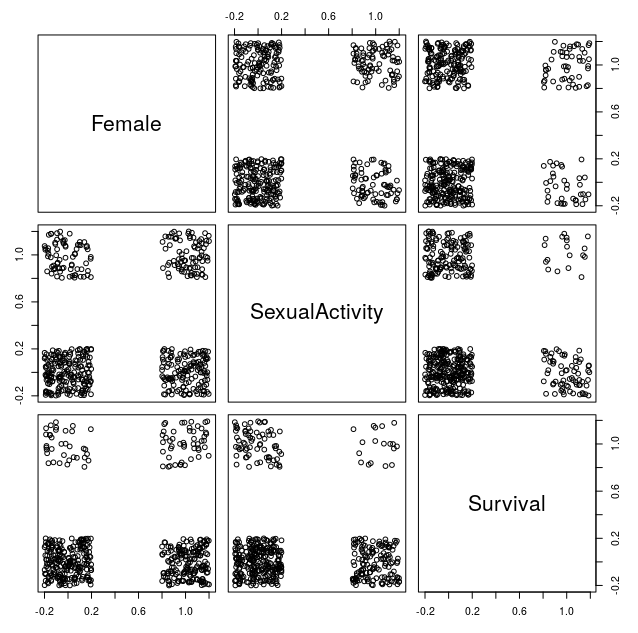
\includegraphics[width=0.5\textwidth]{media/pairs.png}
    \caption{Relationships between variables. Values have been jiggled, since all of them only assume 0 or 1 values.}
    \label{fig:pairs}
    \end{figure}

\section{Model}
Since we have a binary response variable, a logistic regression method is appropriate. We model the survival of character $i$, $y_i$, as a Bernoulli distribution with parameter $p_i$. Each $p_i$ is in turn, a function of the explanatory variables---Gender and Involvement in Sexual Activity---and learnable $\beta$ parameters. We add an interaction variable that is the product of Gender and Involvement in Sexual Activity in order to directly measure the interaction between such variables. Thus, the model has the following specification:
\begin{align}
    y_i | p_i &\stackrel{ind}{\sim} \text{Bern}(p_i),~i=1,\dots,n\\
    p_i &= \frac{1}{1+\text{exp}\left[-\left(\beta_0 + \beta_1G_i + \beta_2S_i + \beta_3\text{int}_i\right)\right]}\\
    \beta_j &\stackrel{i.i.d.}{\sim} \text{Normal}(0, 25),~j=0,\dots,3 \,,
\end{align}
where $G_1$, $S_i$ and $int_i$ are the Gender, Involvement in Sexual Activity and interaction variables of character $i$, respectively. Since the beta parameters give us a measure of how much each explanatory variable affects expectation of survival, this model allow us to answer the research questions.

As priors for the beta coefficients we chose a normal prior with mean 0 and variance 25. This prior is fairly noninformative for logistic regression, due to the sigmoid function. A noninformative prior is chosen to reflect our lack of strong a priori beliefs.

We fit the model using RJAGS. We fit 3 chains for 6000 iterations, filtering out the first 1000 as the burn-in period. This seemed to be sufficient for convergence (potential scale reduction factors of 1 for all parameters, and autocorrelation approaching zero). Figure~\ref{fig:predictions} plots our model predictions against the actual outcomes

\begin{figure}[hbtp]  
    \centering
    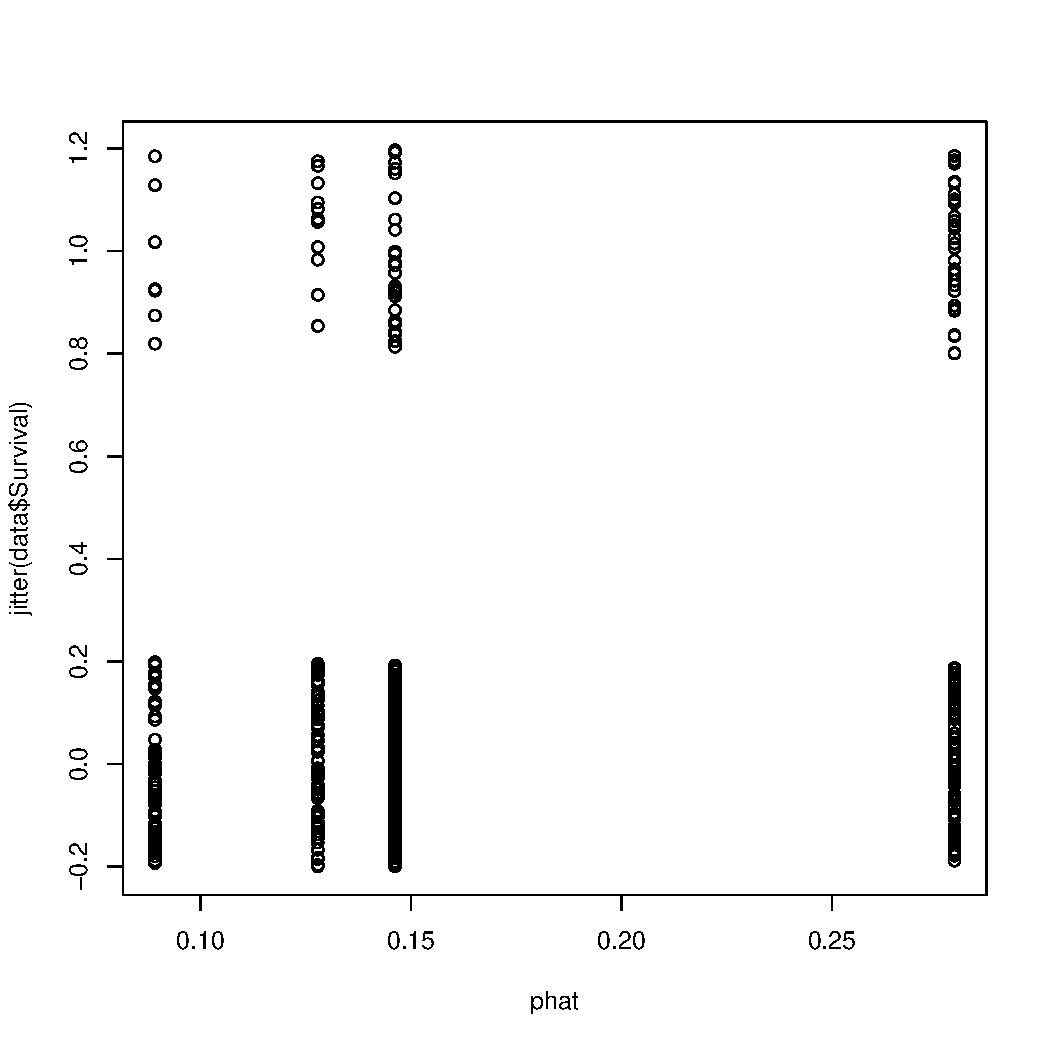
\includegraphics[width=0.5\textwidth]{media/predXlab.pdf}
    \caption{Predictions on the the X axis versus actual outcomes (originally 0 or 1, values were jiggled) on the Y axis. The predictions are sensible, since an increase on phat (expectation of survival) is associated with an increase on the number of surviving characters.}
    \label{fig:predictions}
    \end{figure}

We also trained an alternative model with no interaction variable, which yielded a slightly lower Deviance Information Criterion (DIC)---441.3 against the original model's 442.7. But since we wish to model the interaction between gender and sexual activity, we analyse the original model.

\section{Results}\label{results}
Table~\ref{tab:results} summarises the results. We use the obtained parameter samples to compute the probability of each variable affecting survival chance. We do so by measuring the probability of the parameter being less than zero (negative association with survival chance) or greater than zero (positive association). We find that: we are 99.87\% confident that being female raises survival chance; we are 89.12\% confident that being involved in sexual activity lowers survival chance; we are 76.17\% confident that being involved with sexual activities while being female is even worse and further decreases survival chance when compared to male characters involved in sexual activities.

\begin{table}[hbtp]
    \centering
    \footnotesize
    \caption{Highest posterior density intervals for each parameter (95 \% credibility) and mean estimates.}
    \label{tab:results}
    \begin{tabularx}{\textwidth}{X X X r}
        \toprule
        $\beta_0$ & $\beta_1$ & $\beta_2$ & $\beta_3$\\
        \midrule 
        (-2.19, -1.39), -1.76,  & (0.29, 1.37), 0.82 & (-1.55, 0.79), -0.56& (-2.81, -1.38), -0.41 \\
        \bottomrule
       \end{tabularx}
\end{table}



\section{Conclusions}\label{conclusions}
Our experiments support the following conclusions: i) we are extremely confident that being a woman not involved with sexual activities gives the greatest chance of survival (supporting the ``Final Girl'' hypothesis); ii) we are very confident that being involved in sexual activities reduces the chance of survival; and iii) we are fairly confident that women involved in sexual activities are more harshly punished (with decrease of survival chance) than men.

Our model has the following shortcomings: i) The scarcity of explanatory variables, as the ones we do have are not sufficient to predict if a character lives or dies (in fact, our model always predicts death if we use a cutoff value of 0.5, which is consistent with our data, since all four character groups mostly die---even the women not involved with sexual activity); and ii) lack of granularity of sexual activity, as this variable assume only binary values (even nudity is considered a sexual activity). Other features such as age and profession and a variable with higher granularity of degrees of involvement with sexual activity could better explain survival variability.


\end{document}